\subsection{Thiết kế kiến trúc}
\subsubsection{Lựa chọn kiến trúc}
Hệ thống thương mại điện tử tích hợp Trợ lý Ảo AI của nhóm yêu cầu một kiến trúc \textbf{hiện đại, linh hoạt và có khả năng mở rộng}, đủ để xử lý lượng lớn yêu cầu đồng thời, hỗ trợ phản hồi theo thời gian thực (real-time) và dễ dàng mở rộng theo từng phần.

Từ những phân tích về nhu cầu kỹ thuật và khả năng phát triển lâu dài, kiến trúc hệ thống cần đáp ứng các mục tiêu sau:
\begin{itemize}
    \item Mở rộng linh hoạt cho từng dịch vụ độc lập.
    \item Hỗ trợ xử lý bất đồng bộ và realtime.
    \item Đảm bảo tính cô lập giữa các thành phần.
    \item Cho phép triển khai, cập nhật, bảo trì riêng từng dịch vụ mà không ảnh hưởng toàn hệ thống.
    \item Duy trì độ tin cậy cao, tránh tình trạng “sập dây chuyền” khi một dịch vụ gặp lỗi.
    \item Tận dụng hạ tầng Cloud để tự động hóa triển khai, cân bằng tải và tối ưu chi phí.
    \item Hỗ trợ tích hợp Trợ lý Ảo một cách dễ dàng.
\end{itemize}

\begin{table}[H]
    \centering
    \renewcommand{\arraystretch}{1.4}
    \small
    \begin{tabularx}{\textwidth}{|p{4.5cm}|X|X|X|}
        \hline
        \textbf{Tiêu chí theo yêu cầu hệ thống}               &
        \textbf{Monolithic Architecture}                      &
        \textbf{Microservices Architecture}                   &
        \textbf{Event-Driven + Cloud-Native Architecture}                             \\
        \hline

        Khả năng mở rộng từng chức năng độc lập               &
        Thấp. Toàn bộ hệ thống phải scale cùng nhau           &
        Có thể scale theo từng service                        &
        Cao. Các service và consumer có thể scale độc lập theo tải thực tế            \\
        \hline

        Hỗ trợ xử lý bất đồng bộ và realtime                  &
        Hạn chế, chủ yếu xử lý đồng bộ                        &
        Có hỗ trợ nhưng cần cơ chế giao tiếp bổ sung          &
        Tốt, phù hợp cho xử lý event realtime và message-driven workflow              \\
        \hline

        Tính cô lập giữa các thành phần                       &
        Thấp. Lỗi ở một module dễ ảnh hưởng toàn hệ thống     &
        Tốt hơn nhờ tách service                              &
        Cao. Các service hoạt động độc lập thông qua event broker                     \\
        \hline

        Khả năng triển khai và cập nhật riêng từng thành phần &
        Khó triển khai riêng lẻ                               &
        Có thể triển khai từng service độc lập                &
        Tốt. Hỗ trợ CI/CD và rolling deployment hiệu quả trên Cloud                   \\
        \hline

        Độ tin cậy và khả năng chịu lỗi                       &
        Thấp. Dễ xảy ra lỗi dây chuyền                        &
        Trung bình                                            &
        Cao nhờ cơ chế phân tán và bất đồng bộ                                        \\
        \hline

        Khả năng tận dụng hạ tầng Cloud                       &
        Hạn chế                                               &
        Có hỗ trợ                                             &
        Tốt. Phù hợp với container orchestration, auto scaling và load balancing      \\
        \hline

        Hỗ trợ tích hợp AI Agent                              &
        Khó tích hợp và mở rộng riêng AI service              &
        Có thể triển khai AI thành service riêng              &
        Phù hợp. AI Agent có thể hoạt động như service độc lập và giao tiếp qua event \\
        \hline

        Khả năng mở rộng trong tương lai                      &
        Hạn chế khi hệ thống lớn dần                          &
        Khá tốt                                               &
        Tốt, phù hợp với hệ thống phân tán quy mô lớn                                 \\
        \hline

        Độ linh hoạt trong phát triển và bảo trì              &
        Thấp                                                  &
        Trung bình                                            &
        Cao                                                                           \\
        \hline

        Mức độ phù hợp với đề tài                             &
        Thấp                                                  &
        Khá phù hợp                                           &
        Phù hợp nhất                                                                  \\
        \hline
    \end{tabularx}
    \caption{So sánh các kiến trúc hệ thống theo yêu cầu của đề tài}
    \label{tab:architecture-comparison}
\end{table}

Sau khi tìm hiểu, nghiên cứu về cơ sở lý thuyết của các mô hình kiến trúc phổ biến như \textit{Monolithic}, \textit{Microservices} và \textit{EDA + Cloud-Native}, nhóm lựa chọn kiến trúc \textbf{EDA + Cloud-Native} vì những lý do sau:
\begin{itemize}
    \item Phù hợp với hệ thống có nhiều sự kiện phát sinh và cần xử lý bất đồng bộ như hệ thống thương mại điện tử.
    \item Đảm bảo khả năng phản hồi nhanh và độ trễ thấp.
    \item Dễ dàng mở rộng hoặc thêm mới dịch vụ mà không ảnh hưởng hệ thống hiện hữu.
    \item Giúp giảm phụ thuộc giữa các thành phần và tăng tính mở rộng.
    \item Cho phép tích hợp AI Agent hoạt động với các nền tảng vector database và graph database một cách dễ dàng.
\end{itemize}









\subsubsection{Các lựa chọn thiết kế trong kiến trúc EDA + Cloud-Native}
Các mô hình thiết kế (pattern) trong kiến trúc EDA + Cloud-Native là những mô hình được thiết kế để giúp các dịch vụ giao tiếp và phản ứng với nhau thông qua các sự kiện một cách bất đồng bộ, hiểu quả và an toàn. Cách tiếp cận này giúp xây dựng hệ thống có khả năng mở rộng cao, độ chịu lỗi tốt và mức độ phụ thuộc thấp giữa các thành phần. Những mô hình này mô tả cách sự kiện được tạo ra, truyền đi và tiêu thụ trong môi trường phân tán, qua đó đáp ứng các yêu cầu về khả năng mở rộng theo tải, độ tin cậy, và tính phản hồi của hệ thống.

Các mô hình tiêu biểu gồm Publish–Subscribe, Message Queue, Event Sourcing, CQRS, Saga và Choreography\cite{c4-eda}, mỗi mô hình giải quyết một nhóm vấn đề đặc thù trong quá trình thiết kế và vận hành hệ thống theo kiến trúc EDA + Cloud-Native.






\textbf{Về mặt luân chuyển sự kiện}

Các mô hình luân chuyển sự kiện (Event-Delivery Patterns) mô tả cách sự kiện được truyền từ dịch vụ phát sinh (producer) đến dịch vụ xử lý (consumer). Hai mô hình phổ biến nhất là Publish--Subscribe (Pub/Sub) và Message Queue (MQ). Các cơ chế này giúp hệ thống duy trì sự tách biệt giữa các dịch vụ, đảm bảo độ tin cậy và khả năng mở rộng khi vận hành trên hạ tầng phân tán.

Publish -- Subscribe (Pub/Sub) là mô hình truyền sự kiện trong đó producer gửi sự kiện lên một kênh (topic), và nhiều consumer có thể đồng thời nhận được sự kiện này. Mô hình này giúp hệ thống linh hoạt hơn và dễ mở rộng. Mô hình này có những đặc điểm sau:
\begin{itemize}
    \item Producer không cần biết số lượng hay danh tính consumer\cite{c4-eda}.
    \item Một sự kiện có thể kích hoạt nhiều dịch vụ cùng lúc\cite{c4-eda}.
    \item Mô hình topic hỗ trợ mở rộng theo chiều ngang.
    \item Thích hợp với xử lý song song nhiều luồng.
\end{itemize}
Pub/Sub được ứng dụng trong các hệ thống cần phân phối sự kiện đến nhiều dịch vụ cùng lúc, đặc biệt khi nhiều thành phần trong kiến trúc phải phản ứng đồng thời với các thay đổi. Mô hình này hỗ trợ mở rộng linh hoạt, giảm phụ thuộc giữa các dịch vụ và cho phép xử lý song song ở quy mô lớn, nhờ đó phù hợp với những luồng nghiệp vụ đòi hỏi khả năng phản ứng tức thời và lan tỏa.

Message Queue là mô hình hàng đợi giúp đảm bảo mỗi thông điệp chỉ được xử lý bởi một consumer, phù hợp với mô hình truyền sự kiện điểm--đến--điểm (point--to--point). Đặc điểm của mô hình này là:
\begin{itemize}
    \item Mỗi message được một consumer duy nhất xử lý\cite{c4-eda}.
    \item Không mất message nhờ cơ chế lưu trữ tạm.
    \item Hỗ trợ retry khi lỗi xảy ra.
    \item Giúp phân phối tải giữa nhiều worker.
\end{itemize}
Message Queue được sử dụng trong các nghiệp vụ yêu cầu xử lý tuần tự, đảm bảo tính tin cậy và mức độ cam kết cao trong việc tiêu thụ sự kiện. Mô hình này giúp duy trì sự ổn định của hệ thống bằng cách kiểm soát tải, đảm bảo mỗi sự kiện được xử lý trọn vẹn, đồng thời hạn chế rủi ro mất mát dữ liệu khi dịch vụ gặp sự cố hoặc gián đoạn.

Sau khi phân tích hai mô hình truyền sự kiện phổ biến là Publish/Subscribe và Message Queue, nhóm quyết định lựa chọn Pub/Sub làm mô hình luân chuyển sự kiện cho hệ thống. Việc lựa chọn này xuất phát từ đặc thù của hệ thống thương mại điện tử, nơi mỗi sự kiện thường cần được nhiều dịch vụ cùng lúc lắng nghe và xử lý. Ví dụ, khi một đơn hàng được tạo ra (order\_created), Inventory Service cần cập nhật tồn kho, Payment Service tiếp nhận để xử lý thanh toán, Notification Service gửi thông báo cho người dùng, và Analytics Service ghi nhận dữ liệu phục vụ thống kê. Với Pub/Sub, dịch vụ phát sinh sự kiện không cần biết có bao nhiêu dịch vụ quan tâm, và mỗi consumer có thể xử lý độc lập mà không ảnh hưởng đến phần còn lại của hệ thống.

Mô hình Pub/Sub giúp giảm mạnh sự phụ thuộc giữa các dịch vụ và tạo điều kiện cho việc mở rộng hệ thống về sau. Khi bổ sung dịch vụ mới, chỉ cần đăng ký (subscribe) vào topic sự kiện mà không cần thay đổi bất kỳ thành phần đang hoạt động. Điều này phù hợp với tư duy mở rộng linh hoạt của kiến trúc Cloud-Native và giúp hệ thống vận hành bất đồng bộ hiệu quả. Vì các lợi ích trên, nhóm thống nhất lựa chọn Pub/Sub làm mô hình truyền sự kiện duy nhất cho toàn bộ hệ thống.
\bigskip






\textbf{Về mặt quản lý trạng thái dữ liệu}

Trong môi trường phân tán, quản lý trạng thái dữ liệu đóng vai trò then chốt. Do đó, để hạn chế sự bất đồng bộ trong trạng thái dữ liệu giữa các dịch vụ, chúng ta cần thiết kế hệ thống theo các mô hình quản lý trạng thái (State Management Patterns) hiện đại và phù hợp. Hai mô hình thông dụng là Event Sourcing và CQRS, mỗi mô hình phù hợp cho các loại nghiệp vụ khác nhau.

Event Sourcing lưu toàn bộ thay đổi dưới dạng chuỗi sự kiện thay vì trạng thái cuối cùng. Đặc điểm của mô hình này là:
\begin{itemize}
    \item Lưu lịch sử dữ liệu đầy đủ\cite{c4-eda}.
    \item Khôi phục trạng thái bằng replay sự kiện.
    \item Hỗ trợ kiểm toán và truy vết mạnh\cite{c4-eda}.
    \item Yêu cầu thiết kế và lưu trữ phức tạp hơn\cite{c4-eda}.
\end{itemize}
Event Sourcing thích hợp cho các hệ thống cần duy trì lịch sử thay đổi chi tiết, hỗ trợ kiểm toán hoặc phục hồi trạng thái với độ chính xác cao. Nhờ lưu lại toàn bộ chuỗi sự kiện, mô hình này cho phép tái xây dựng dữ liệu, phân tích hành vi theo thời gian và đáp ứng các yêu cầu về minh bạch, nhất quán và khả năng truy vết trong môi trường phân tán.

CQRS (Command Query Responsibility Segregation) tách biệt luồng ghi và luồng đọc, giúp tối ưu từng thành phần riêng biệt. Mô hình này có những đặc điểm sau:
\begin{itemize}
    \item Tách biệt đường đi của đọc và ghi\cite{c4-eda}.
    \item Cho phép tối ưu từng luồng theo nhu cầu\cite{c4-eda}.
    \item Hỗ trợ mở rộng độc lập.
    \item Tăng cường bảo mật nhờ phân tách chức năng.
\end{itemize}
CQRS phù hợp với những hệ thống có tải truy vấn lớn, nơi nhu cầu đọc dữ liệu vượt trội so với ghi. Việc tách biệt hai luồng xử lý giúp tối ưu hiệu năng, cải thiện tốc độ phản hồi và cho phép mở rộng độc lập từng phần của hệ thống, đồng thời tăng cường khả năng kiểm soát truy cập và tính linh hoạt trong thiết kế dữ liệu.

Trong hai mô hình quản lý trạng thái là Event Sourcing và CQRS, nhóm lựa chọn CQRS làm mô hình quản lý trạng thái dữ liệu cho hệ thống. Lý do là hệ thống thương mại điện tử thường có tỷ lệ truy vấn đọc lớn hơn rất nhiều so với tỷ lệ ghi. Người dùng liên tục xem sản phẩm, xem giỏ hàng, xem lịch sử đơn hàng và tra cứu thông tin chi tiết. Các thao tác này yêu cầu phản hồi nhanh, ổn định và có khả năng xử lý tải cao. CQRS cho phép tách phần ghi (command) và phần đọc (query) thành hai thành phần độc lập, giúp tối ưu từng luồng theo đúng đặc thù của nó.

Với CQRS, phần ghi tập trung đảm bảo tính toàn vẹn dữ liệu và xử lý đúng logic nghiệp vụ, trong khi phần đọc có thể được tối ưu bằng cache, denormalized view hoặc cơ sở dữ liệu chuyên biệt cho truy vấn nhanh. Điều này làm giảm tải cho hệ thống ghi và cải thiện tốc độ truy vấn lên giao diện người dùng

Event Sourcing mặc dù mạnh về khả năng lưu vết, nhưng lại phức tạp trong thiết kế và không phù hợp với đề tài của nhóm. Do đó, nhóm chọn CQRS làm mô hình quản lý trạng thái duy nhất để đảm bảo cân bằng giữa hiệu năng, sự đơn giản và khả năng triển khai thực tế.
\bigskip






\textbf{Về mặt điều phối hệ thống}

Các mô hình điều phối (Orchestration Patterns) mô tả cách các dịch vụ phối hợp để xử lý quy trình nghiệp vụ phức tạp. Hai mô hình phổ biến là Saga và Choreography.

Saga chia tác vụ lớn thành nhiều bước nhỏ, mỗi bước có thể rollback khi lỗi xảy ra. Mô hình này có những đặc điểm sau:
\begin{itemize}
    \item Chia tác vụ thành nhiều bước tuần tự.
    \item Có hành động để xử lý lỗi nếu có ở từng bước\cite{c4-eda}.
    \item Có trung tâm điều phối (orchestrator) để tổ chức thực hiện tác vụ\cite{c4-eda}.
    \item Hỗ trợ xử lý lỗi và rollback có kiểm soát.
\end{itemize}
Saga được áp dụng trong các quy trình nghiệp vụ phức tạp đòi hỏi nhiều bước xử lý có liên quan và cần duy trì tính nhất quán trong môi trường phân tán. Mô hình này hỗ trợ điều phối luồng công việc theo từng giai đoạn, đảm bảo hệ thống có thể xử lý lỗi an toàn, khôi phục từng phần khi cần thiết và duy trì tính toàn vẹn của các giao dịch dài.

Choreography không dùng orchestrator; các dịch vụ tự lắng nghe sự kiện và thực thi tương ứng. Đặc điểm của mô hình này là:
\begin{itemize}
    \item Không có bộ điều phối trung tâm\cite{c4-eda}.
    \item Mở rộng tự nhiên theo kiến trúc phân tán.
    \item Khó kiểm soát khi quy trình phức tạp\cite{c4-eda}.
\end{itemize}
Choreography phù hợp với các quy trình nhẹ, mang tính linh hoạt cao và không yêu cầu sự điều phối tập trung. Mỗi dịch vụ phản ứng độc lập theo sự kiện, giúp hệ thống giảm bớt ràng buộc, dễ mở rộng và hoạt động theo hướng phi tập trung. Mô hình này đặc biệt hữu ích trong những luồng nghiệp vụ đơn giản hoặc các tác vụ bổ trợ trong kiến trúc sự kiện.

Trong nhóm các mô hình điều phối nghiệp vụ, sau khi xem xét Saga và Choreography, nhóm quyết định lựa chọn Saga làm mô hình điều phối hệ thống. Quy trình đặt hàng trong thương mại điện tử là quy trình phức tạp, bao gồm nhiều bước phụ thuộc lẫn nhau như kiểm tra tồn kho, xử lý thanh toán, tạo đơn hàng, cập nhật trạng thái và gửi thông báo. Mỗi bước đều có khả năng phát sinh lỗi và yêu cầu cơ chế rollback phù hợp để đảm bảo tính nhất quán của toàn hệ thống.

Saga Orchestration có một orchestrator trung tâm chịu trách nhiệm điều phối từng bước của quy trình, theo dõi trạng thái và quyết định thực hiện hành động bù trừ (compensation) khi xảy ra lỗi. Mô hình này giúp kiểm soát luồng nghiệp vụ rõ ràng, dễ quan sát, dễ debug và phù hợp với yêu cầu thực tế của đề tài. So với Choreography, Saga tránh được tình trạng “event chaos” khi có nhiều dịch vụ phản ứng lẫn nhau, đồng thời mang lại sự minh bạch và khả năng kiểm soát cao hơn.

Vì các lý do trên, nhóm lựa chọn Saga Orchestration làm mô hình điều phối cho toàn bộ các quy trình nghiệp vụ quan trọng trong hệ thống, đặc biệt là quy trình đặt hàng.
\bigskip









\subsubsection{Các tầng của hệ thống}
\begin{figure}[H]
    \centering
    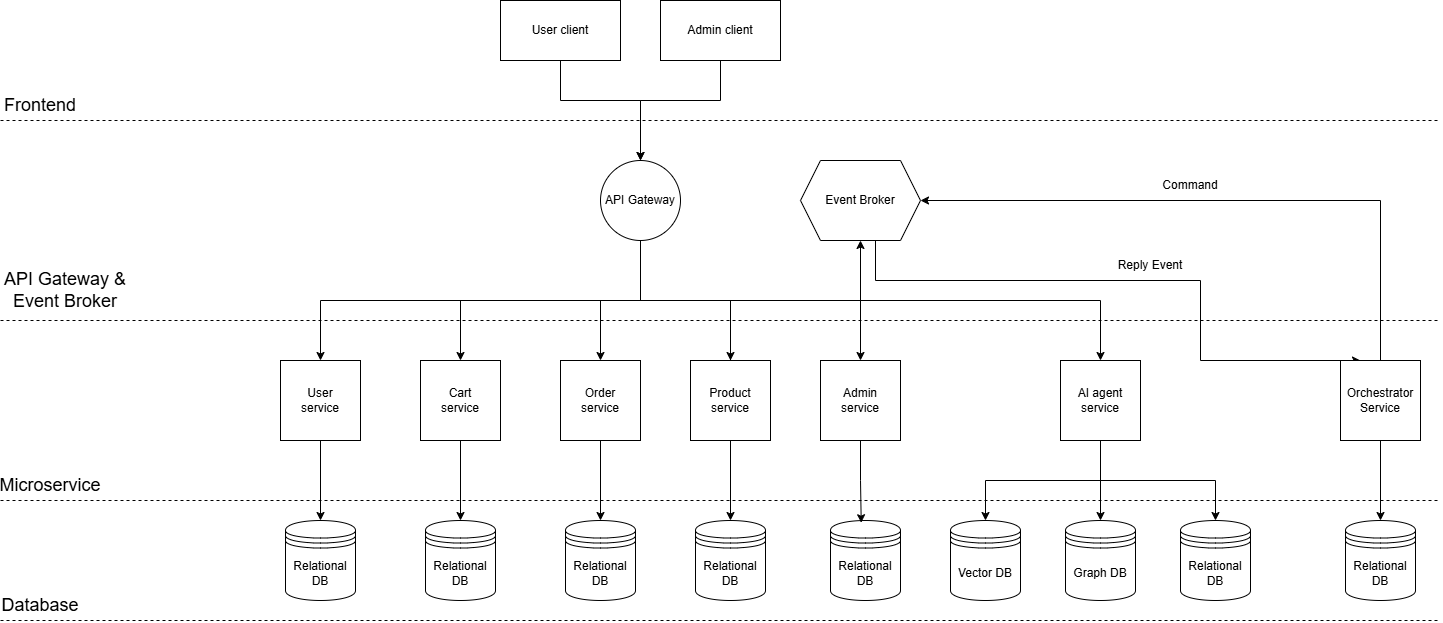
\includegraphics[width=\textwidth]{images/chap6/Architecture diagram.drawio.png}
    \vspace{0.5cm}
    \caption{Sơ đồ kiến trúc hệ thống}
    \label{fig:whole_system_architecture}
\end{figure}

Hình \ref{fig:whole_system_architecture} bên trên biểu diễn kiến trúc tổng thể của hệ thống của nhóm. Sơ đồ \ref{fig:whole_system_architecture} cho thấy hệ thống của nhóm được tổ chức bao gồm bốn tầng chính:
\begin{itemize}
    \item Frontend
    \item API Gateway \& Event Broker
    \item Microservice
    \item Database
\end{itemize}
Mỗi tầng đảm nhiệm một vai trò riêng biệt trong việc xử lý yêu cầu, điều phối hoạt động và lưu trữ dữ liệu.

\textbf{Tầng Frontend}

Tầng Frontend đóng vai trò là điểm tương tác đầu tiên giữa người dùng với hệ thống. Tầng này bao gồm hai thành phần chính: Giao diện dành cho khách hàng (User client) và giao diện dành cho quản trị viên của hệ thống (Admin client). User client là nơi diễn ra toàn bộ các hoạt động của khách hàng như xem sản phẩm, thêm vào giỏ hàng, đặt hàng hoặc theo dõi tình trạng đơn hàng. Trong khi đó, Admin client phục vụ quản trị viên trong việc quản lý danh mục sản phẩm, kiểm soát đơn hàng, điều chỉnh thông tin và xử lý các thao tác vận hành nội bộ.

Cả hai giao diện đều giao tiếp với các phần khác của hệ thống thông qua một thành phần duy nhất là API Gateway, đảm bảo toàn bộ yêu cầu được thống nhất về đường đi và cách xử lý.
\bigskip



\textbf{Tầng API Gateway và Event Broker}

Tầng này bao gồm hai thành phần chính: API Gateway và Event Broker, mỗi thành phần đảm nhiệm một vai trò khác nhau trong cơ chế vận hành của hệ thống.

API Gateway hoạt động như một lớp trung gian giữa Frontend và Microservices. Đây là nơi tiếp nhận tất cả các yêu cầu từ User client và Admin client, sau đó định tuyến chúng đến đúng microservice phía dưới. Việc đặt API Gateway giữa giao diện và các service giúp kiểm soát luồng dữ liệu, hợp nhất các điểm truy cập và tạo điều kiện thuận lợi cho việc áp dụng các chính sách hệ thống trong tương lai như phân quyền, kiểm soát tốc độ và ghi log.

Song song với API Gateway, hệ thống còn sử dụng một Event Broker. Event Broker đảm nhiệm việc truyền tải và phân phối các sự kiện nội bộ giữa các service theo mô hình Publish/Subscribe. Điều này cho phép các microservice xử lý bất đồng bộ, tránh việc phải gọi trực tiếp lẫn nhau và giảm thiểu sự phụ thuộc giữa các module.
\bigskip



\textbf{Tầng Microservice}

Tầng này bao gồm bảy dịch vụ độc lập theo chức năng, trong đó có một service điều phối điều phối Saga để duy trì tính nhất quán dữ liệu trong các giao dịch phân tán, năm service nghiệp vụ thương mại điện tử và một service chuyên biệt về AI được thể hiện rõ trên sơ đồ:
\begin{itemize}
    \item User service: Quản lý thông tin người dùng và các thao tác liên quan đến tài khoản.
    \item Cart service: Xử lý toàn bộ hoạt động liên quan đến giỏ hàng của người dùng.
    \item Order service: Tiếp nhận và xử lý yêu cầu liên quan đến đặt hàng và lưu đơn hàng.
    \item Product service: Lưu trữ và cung cấp thông tin về sản phẩm cho hệ thống.
    \item Admin service: Hỗ trợ các chức năng quản trị.
    \item AI agent service: Thực hiện các hoạt động của Trợ lý Ảo như tư vấn sản phẩm, kiểm tra thông tin, ...
    \item Orchestrator Service: Thực hiện mô hình Saga Orchestration, chuyên trách điều phối các quy trình nghiệp vụ phức tạp bằng cách quản lý Trạng thái Saga, gửi Commands và xử lý Reply Events qua Event Broker. Dịch vụ này có Database riêng để lưu trữ Metadata Điều phối.
\end{itemize}
Các microservice không có bất kỳ liên kết trực tiếp nào với nhau trong sơ đồ, thay vào đó toàn bộ giao tiếp đều phải thông qua Event Broker. Điều này giúp cho mỗi service được vận hành tách biệt, giúp giảm thiểu tình trạng xung đột logic, tăng tính chủ động khi triển khai và bảo trì, và bên cạnh đó còn giúp hỗ trợ nhóm phân chia công việc dễ dàng hơn trong giai đoạn hiện thực hệ thống.

Ngoài ra, về mặt cấu trúc nội bộ, mỗi Microservice nghiệp vụ được nhóm tổ chức theo mô hình phân tầng cơ bản.

\begin{figure}[H]
    \centering
    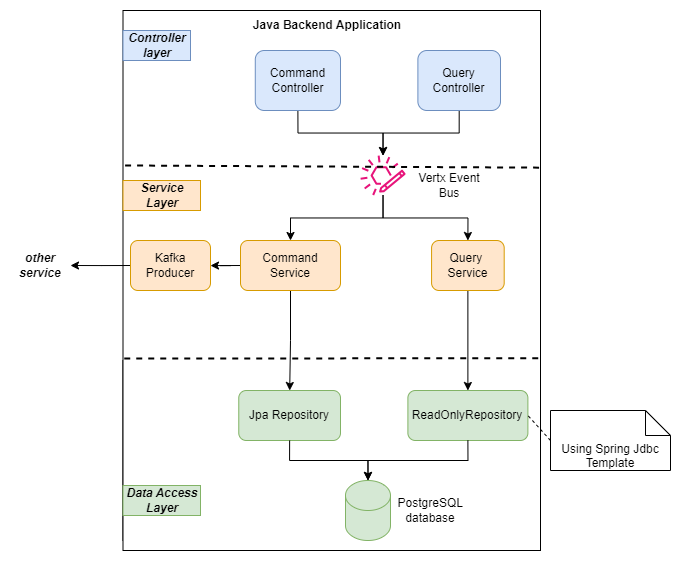
\includegraphics[width=0.85\textwidth]{images/chap6/JavaBackend.png}
    \vspace{0.5cm}
    \caption{Cấu trúc nội bộ Microservice của các dịch vụ Java}
    \label{fig:internal_service_architecture}
\end{figure}
\vspace{-0.5cm}
Sơ đồ \ref{fig:internal_service_architecture} mô tả cấu trúc nội bộ của các dịch vụ nghiệp vụ trong hệ thống. Nhóm sử dụng Vert.x Event Bus làm bộ điều phối nội bộ để chuyển giao các yêu cầu một cách bất đồng bộ. Luồng ghi dùng JPA Repository để quản lý các thực thể phức tạp và đảm bảo tính nhất quán dữ liệu trong cơ sở dữ liệu PostgreSQL. Ngược lại, luồng đọc sử dụng một kho lưu trữ riêng với Spring JdbcTemplate để thực hiện các câu lệnh SQL thuần, giúp loại bỏ độ trễ của các bộ thư viện ánh xạ thực thể và tăng tốc độ phản hồi. Thêm vào đó, Kafka Producer ở luồng ghi sẽ phát đi các sự kiện nghiệp vụ. Đây là mắt xích quan trọng để kích hoạt các quy trình liên dịch vụ như SAGA, đảm bảo tính toàn vẹn dữ liệu cho toàn bộ hệ thống phân tán.

\bigskip

\subsubsection{Cấu trúc nội bộ Frontend}

Tầng Frontend được xây dựng dựa trên framework Next.js 16, áp dụng kiến trúc \textbf{Feature-Sliced Design (FSD)} kết hợp với các tính năng hiện đại của React 19 để tối ưu hóa khả năng bảo trì và hiệu năng.

\begin{figure}[H]
    \centering
    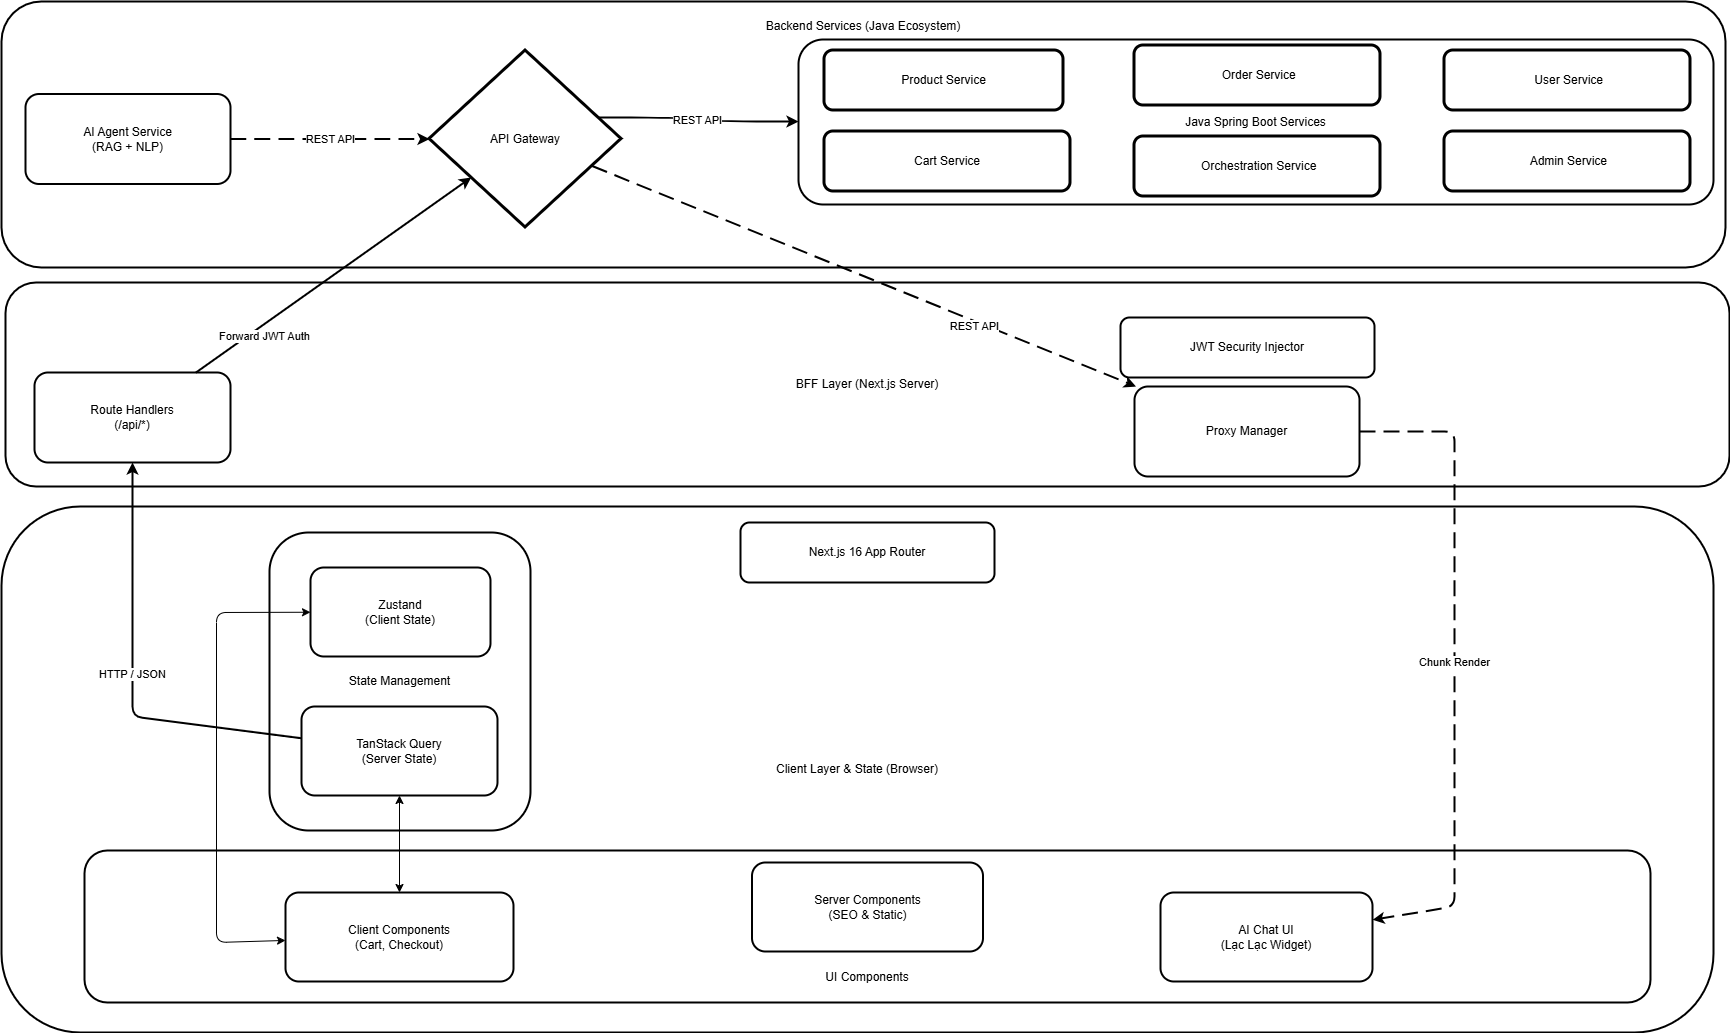
\includegraphics[width=0.85\textwidth]{images/chap4/architecture/frontend_fsd.png}
    \vspace{0.5cm}
    \caption{Cấu trúc nội bộ tầng Frontend}
    \label{fig:frontend_internal_architecture}
\end{figure}

Sơ đồ \ref{fig:frontend_internal_architecture} mô tả các thành phần cốt lõi trong kiến trúc Frontend:

\begin{itemize}
    \item \textbf{App Router \& Server Components:} Next.js App Router quản lý luồng điều hướng và render các Server Components phía máy chủ. Điều này giúp giảm thiểu đáng kể lượng JavaScript tải xuống trình duyệt, đồng thời cho phép lấy dữ liệu (fetching) trực tiếp từ server-side trước khi gửi HTML về cho khách hàng.
    \item \textbf{BFF (Backend for Frontend):} Các Route Handlers của Next.js đóng vai trò là một lớp BFF trung gian. Client-side components không gọi trực tiếp tới các Microservices ở Backend mà thông qua các API routes nội bộ. Lớp này giúp ẩn đi các thông tin nhạy cảm (như API Gateway URL), hợp nhất các lời gọi API và thực hiện các biến đổi dữ liệu cần thiết trước khi trả về UI.
    \item \textbf{Features-based Modules:} Mã nguồn được tổ chức theo các tính năng (features) như \texttt{auth}, \texttt{cart}, \texttt{product}, \texttt{order} và \texttt{chat-ai}. Mỗi module chứa đầy đủ các thành phần (components), trạng thái (store), và hooks riêng biệt, giúp tăng tính cô lập và dễ dàng mở rộng.
    \item \textbf{State Management Partitioning:}
          \begin{itemize}
              \item \textbf{Server State:} Sử dụng TanStack Query để quản lý cache, đồng bộ và quản lý vòng đời của dữ liệu từ backend.
              \item \textbf{Client State:} Sử dụng Zustand để quản lý các trạng thái cục bộ mượt mà, không gây re-render dư thừa.
          \end{itemize}
    \item \textbf{AI Chat Integration:} Thành phần Chatbot được thiết kế để giao tiếp với AI Agent Service thông qua các giao thức RESTful tiêu chuẩn. Hệ thống sử dụng các thư viện quản lý yêu cầu (fetching) để gửi câu hỏi từ người dùng dưới dạng JSON và nhận về phản hồi đã được xử lý hoàn chỉnh từ Backend, giúp đảm bảo tính đồng bộ và dễ dàng quản lý lịch sử hội thoại tại Client State.
\end{itemize}


\bigskip

\textbf{Tầng Database}

Tầng Database chịu trách nhiệm lưu trữ dữ liệu cho từng microservice. Mỗi microservice có cơ sở dữ liệu riêng của nó:
\begin{itemize}
    \item User service → Lưu trữ toàn bộ thông tin người dùng và dữ liệu tài khoản liên quan.
    \item Cart service → Lưu dữ liệu giỏ hàng của từng người dùng, bao gồm danh sách và số lượng sản phẩm.
    \item Order service → Lưu thông tin đơn hàng, trạng thái xử lý và các dữ liệu liên quan đến quá trình đặt hàng.
    \item Product service → Lưu trữ danh sách sản phẩm, thuộc tính và thông tin mô tả sản phẩm.
    \item Admin service → Lưu dữ liệu phục vụ thao tác quản trị và điều chỉnh thông tin hệ thống.
    \item AI agent service → Lưu trữ các thông tin về thông số của các sản phẩm, cũng như các vector embedding dùng cho xử lý truy vấn và gợi ý của Trợ lý Ảo. Bên cạnh đó, lưu các quan hệ dạng đồ thị giữa sản phẩm, hành vi và dữ liệu cần phân tích cho Trợ lý Ảo.
    \item Orchestrator service → Lưu trữ metadata điều phối Saga, bao gồm trạng thái hiện tại của các Saga đang chạy, thông tin về các bước đã hoàn thành và các dữ liệu cần thiết để quản lý quy trình nghiệp vụ phân tán.
\end{itemize}
Các service chính như User, Cart, Order, Product và Admin đều sử dụng cơ sở dữ liệu quan hệ, đảm bảo lưu trữ dữ liệu theo cấu trúc bảng truyền thống.

Riêng AI agent service sở hữu ba cơ sở dữ liệu độc lập: cơ sở dữ liệu quan hệ, cơ sở dữ liệu Vector và cơ sở dữ liệu Graph, tương ứng với ba loại dữ liệu mà service này cần quản lý. Điều này cho phép dịch vụ Trợ lý Ảo vận hành trên những tập dữ liệu phù hợp với nhu cầu xử lý của nó.


\subsubsection{Kiến trúc thành phần}
\begin{figure}[H]
    \centering
    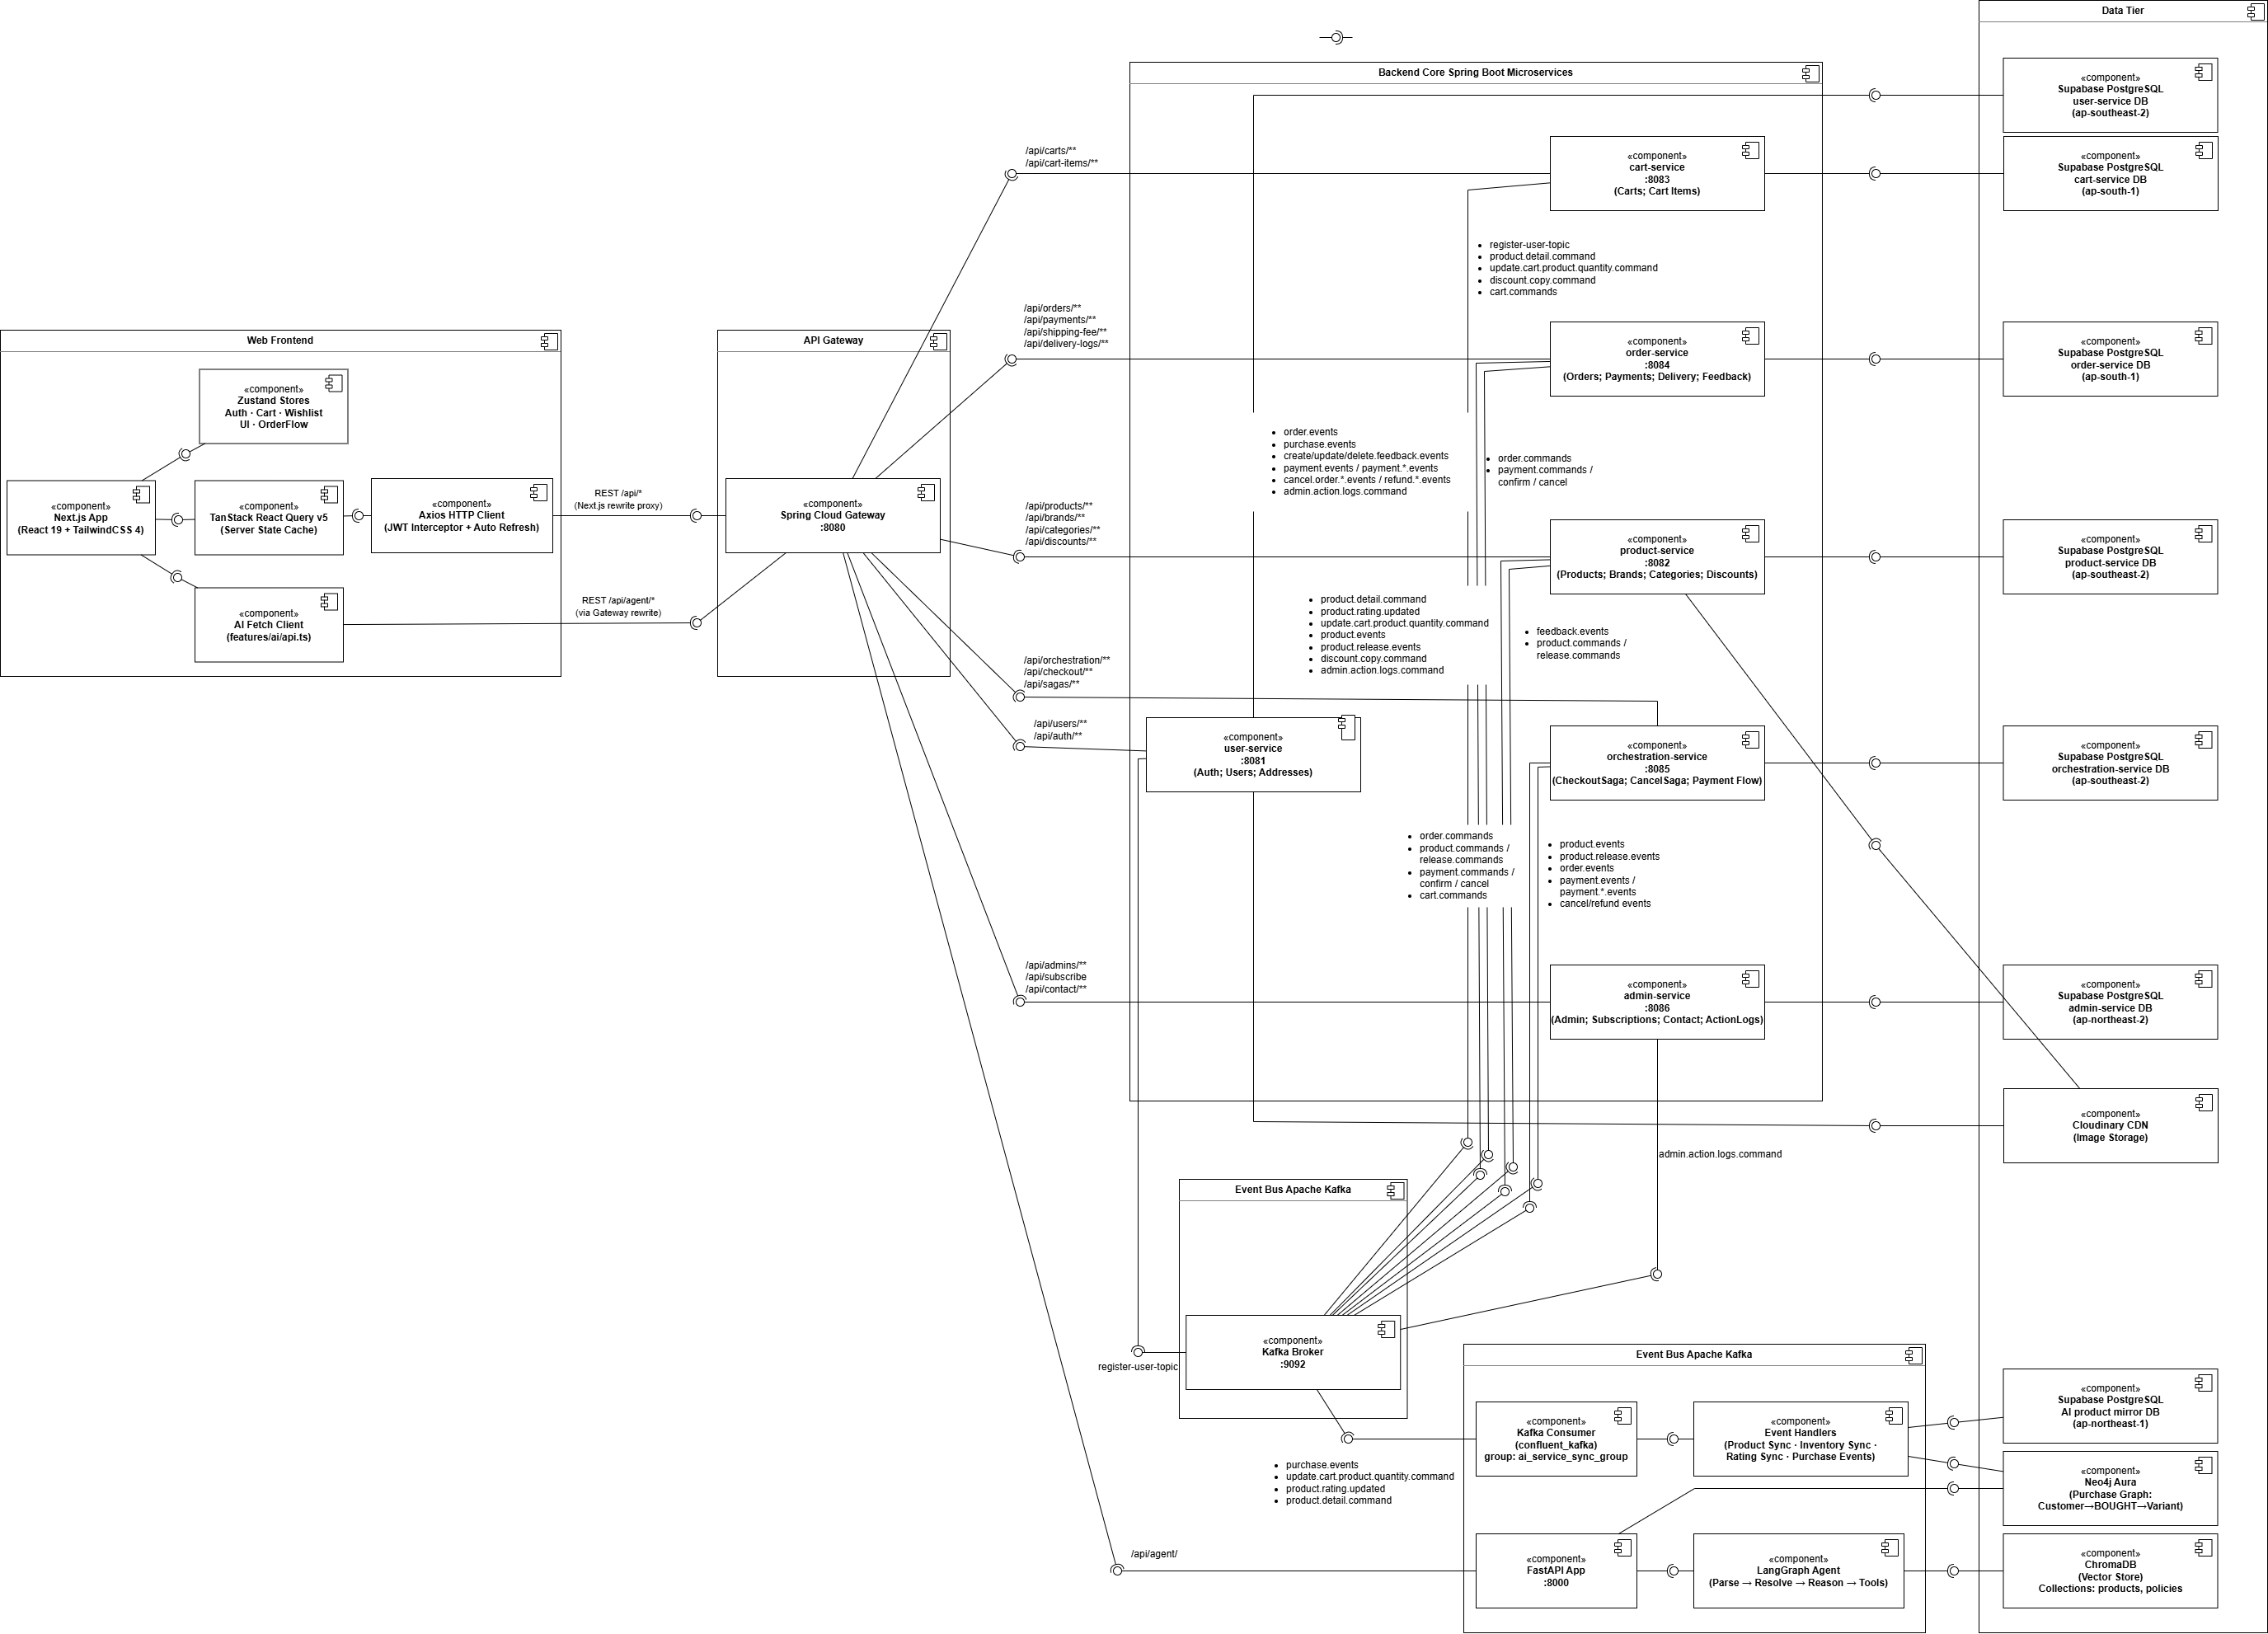
\includegraphics[width=\textwidth]{images/chap6/component-diagram.png}
    \vspace{0.5cm}
    \caption{Sơ đồ thành phần kiến trúc hệ thống}
    \label{fig:component_diagram}
\end{figure}

Sơ đồ \ref{fig:component_diagram} biểu diễn các thành phần công nghệ cốt lõi và luồng giao tiếp thực tế của hệ thống. Do giới hạn kích thước hiển thị trong tài liệu, phiên bản đầy đủ với độ phân giải cao được cung cấp tại \href{https://drive.google.com/file/d/1qQgxTPdSjFGyEHMbc9x7tZ9cWqRHhKW-/view?usp=drive_link}{liên kết đính kèm} nhằm hỗ trợ việc quan sát các thành phần rõ ràng hơn. Do vai trò và chức năng nghiệp vụ của các tầng đã được trình bày chi tiết ở mục trước, phần này tập trung tóm tắt các công nghệ và nền tảng chính được áp dụng cho từng thành phần:

\begin{itemize}
    \item \textbf{Tầng giao diện người dùng (Frontend):} Phát triển trên nền tảng Next.js 16 (React 19). Ứng dụng Zustand để quản lý Client State và TanStack React Query cho Server State. Giao tiếp mạng được xử lý qua Axios với cơ chế tự động làm mới token.
    \item \textbf{Tầng API Gateway:} Sử dụng Spring Cloud Gateway (cổng 8080) làm điểm định tuyến tập trung và bảo vệ các dịch vụ nội bộ (microservices).
    \item \textbf{Tầng Backend Core:} Các dịch vụ nghiệp vụ cốt lõi được xây dựng bằng framework Spring Boot.
    \item \textbf{Tầng AI Agent (Trợ lý Ảo):} Tách biệt hoàn toàn dưới dạng dịch vụ độc lập viết bằng Python FastAPI, sử dụng LangGraph và LangChain làm động cơ AI (AI Engine). Hệ thống AI đồng bộ dữ liệu thời gian thực từ Backend Core thông qua Kafka Consumer.
    \item \textbf{Tầng Event Bus (Điều phối sự kiện):} Apache Kafka hoạt động như trục xương sống trao đổi thông điệp bất đồng bộ, hiện thực hóa các mô hình phân tán như Saga Orchestration và CQRS.
    \item \textbf{Tầng Database (Lưu trữ dữ liệu):} Áp dụng mô hình Database-per-Service. Dữ liệu quan hệ được lưu trữ tại Supabase PostgreSQL. Dịch vụ AI sử dụng kết hợp Neo4j Aura (Graph Database) và ChromaDB (Vector Database) phục vụ phân tích ngữ nghĩa. Hình ảnh và phương tiện truyền thông được quản lý qua Cloudinary CDN.
\end{itemize}
\bigskip

\subsubsection{Kiến trúc triển khai}
\begin{figure}[H]
    \centering
    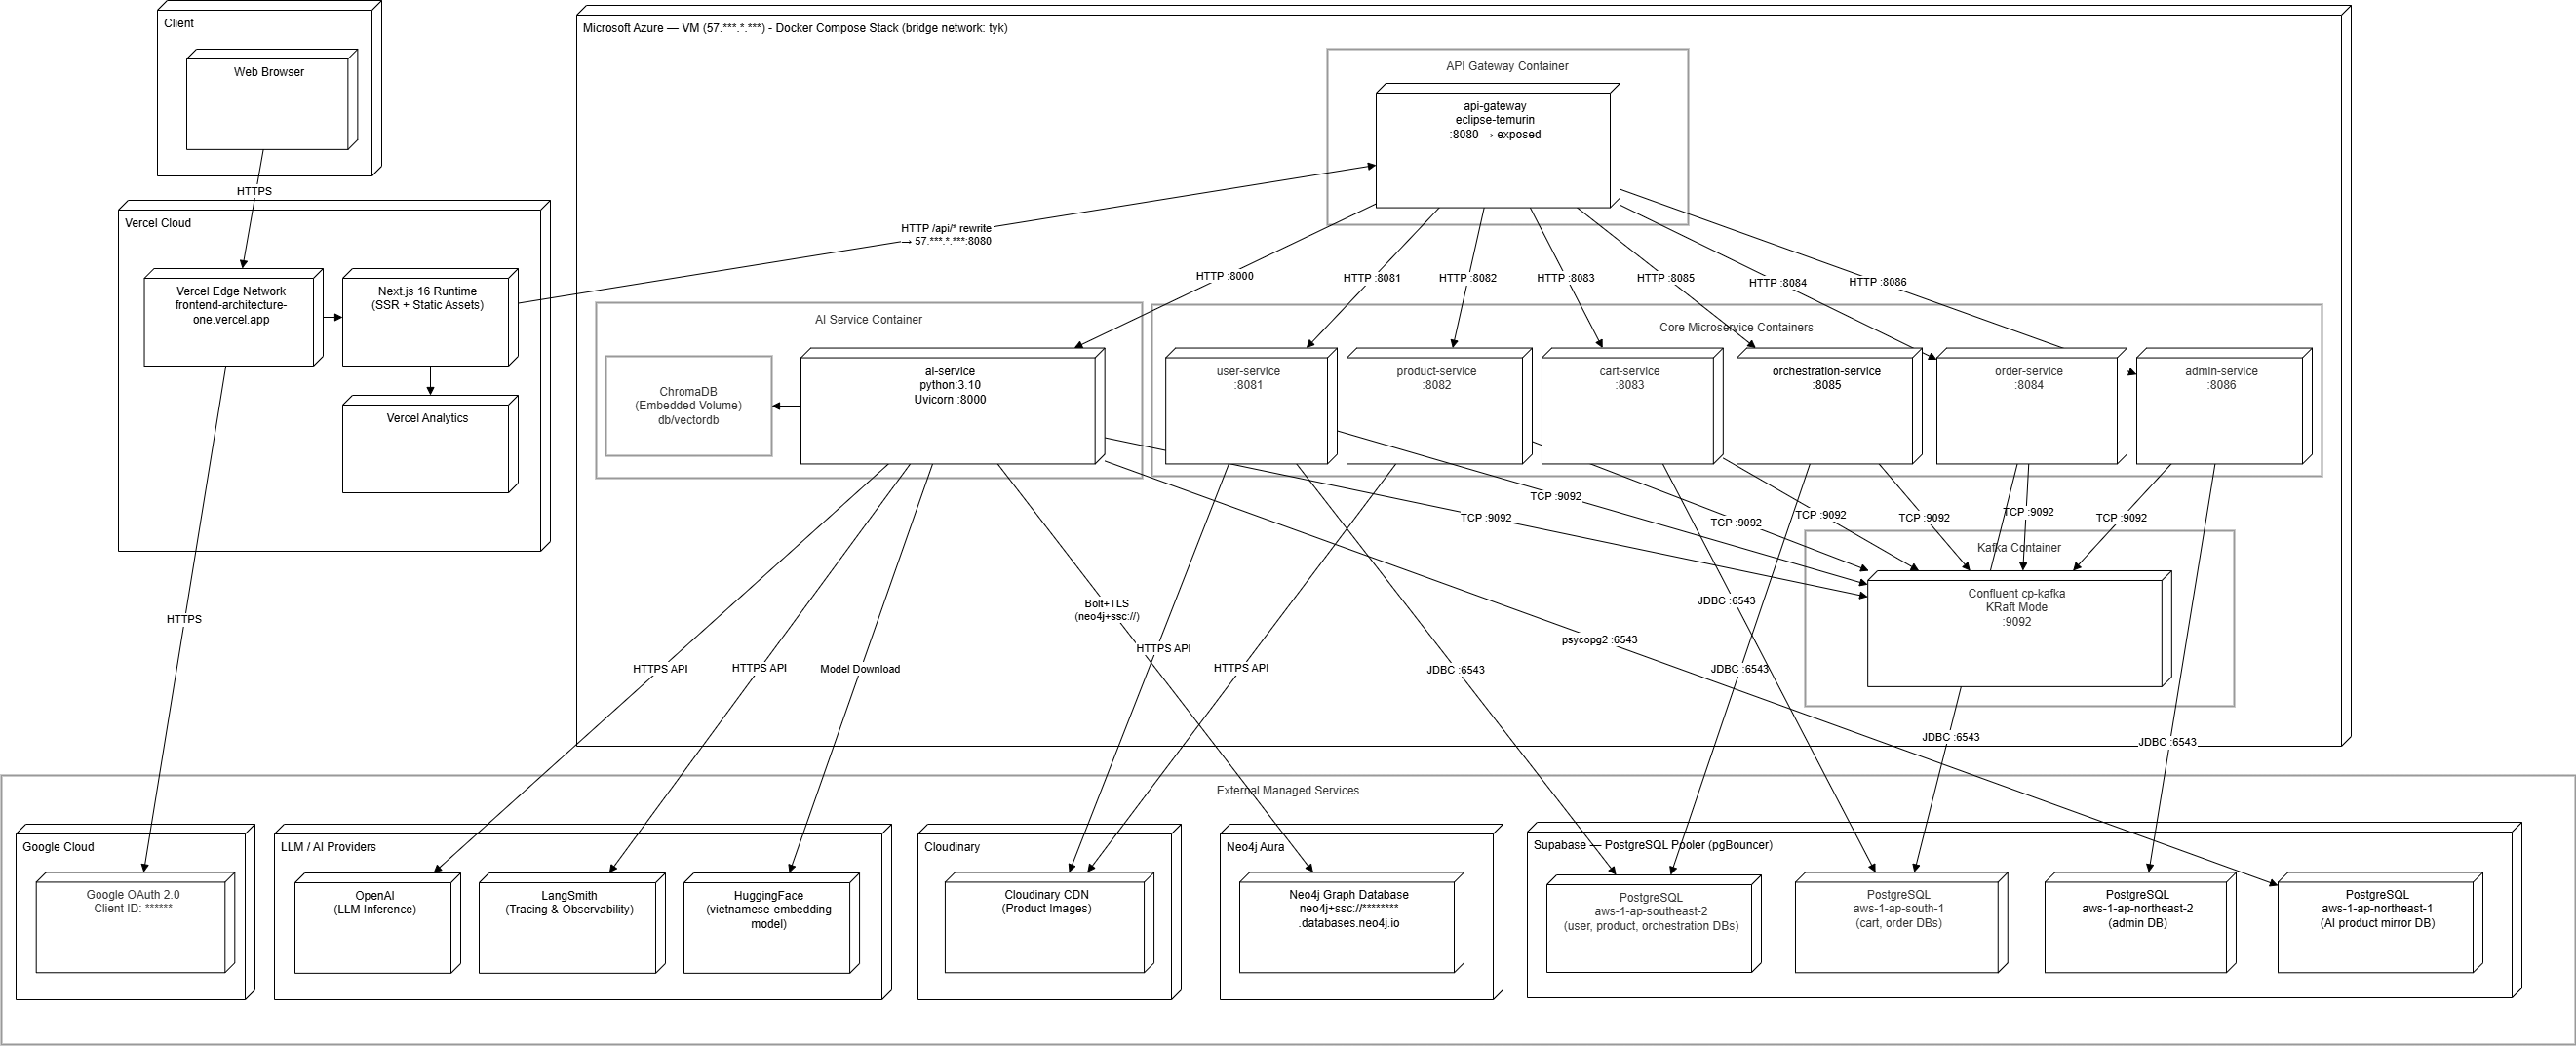
\includegraphics[width=\textwidth]{images/chap6/deployment-diagram.png}
    \vspace{0.5cm}
    \caption{Sơ đồ triển khai hệ thống}
    \label{fig:deployment_diagram}
\end{figure}

Sơ đồ \ref{fig:deployment_diagram} thể hiện chi tiết cách thức các thành phần của hệ thống được phân bổ, kết nối và triển khai thực tế trên hạ tầng mạng. Do giới hạn kích thước hiển thị trong tài liệu, phiên bản đầy đủ với độ phân giải cao được cung cấp tại \href{https://drive.google.com/file/d/1qfIlCt7C07wGTaG6CrbSDzNkafoRDNpT/view?usp=drive_link}{liên kết đính kèm} nhằm hỗ trợ việc quan sát các thành phần rõ ràng hơn. Kiến trúc triển khai này mô tả chân thực cấu trúc vật lý của hệ thống, tận dụng sức mạnh của các dịch vụ đám mây được quản lý (Managed Services) kết hợp cùng kỹ thuật đóng gói vùng chứa (Containerization).

\textbf{Khối Vercel Cloud (Frontend Hosting)}

Mã nguồn Frontend (Next.js) được triển khai trực tiếp lên mạng lưới Vercel Edge. Việc triển khai này tận dụng khả năng Server-Side Rendering (SSR) mạnh mẽ và phân phối tĩnh (Static Assets) qua CDN toàn cầu của Vercel, mang lại tốc độ truy cập cực nhanh cho khách hàng. Vercel Analytics cũng được tích hợp sẵn để theo dõi và đánh giá hiệu suất phía giao diện người dùng.
\bigskip

\textbf{Khối Microsoft Azure VM (Backend Hosting)}

Toàn bộ hệ sinh thái Microservices (bao gồm 6 dịch vụ Spring Boot, 1 dịch vụ FastAPI AI, API Gateway và Apache Kafka) được đóng gói thành các container Docker và điều phối cục bộ bằng công cụ \textbf{Docker Compose} trên một máy chủ ảo (Virtual Machine) duy nhất thuộc nền tảng Microsoft Azure (với địa chỉ IP: 57.155.2.144).
\begin{itemize}
    \item \textbf{Mạng cục bộ (Bridge Network):} Các container giao tiếp an toàn qua một mạng nội bộ chung có tên là \texttt{tyk}. Kiến trúc này không mở cổng (port) trực tiếp ra bên ngoài, ngoại trừ cổng 8080 của API Gateway, giúp tối ưu hóa khả năng bảo vệ hệ thống trước các truy cập trái phép.
    \item \textbf{Kafka Broker:} Hệ thống sử dụng Confluent Kafka (\texttt{cp-kafka:7.8.0}) chạy ở chế độ KRaft (không phụ thuộc vào Zookeeper). Đây là một container tự lưu trữ (self-hosted) ngay trong VM, góp phần giảm thiểu đáng kể độ trễ nội bộ khi truyền tải Luồng sự kiện (Event stream) giữa các dịch vụ so với việc sử dụng hệ thống Kafka ngoại vi trên đám mây.
\end{itemize}
\bigskip

\textbf{Khối dịch vụ đám mây ngoại vi (External Managed Services)}

Thay vì tự quản trị toàn bộ hệ quản trị cơ sở dữ liệu, hệ thống khai thác tối đa mô hình dịch vụ đám mây để đảm bảo độ an toàn và khả năng sao lưu:
\begin{itemize}
    \item \textbf{Supabase PostgreSQL Pooler:} Cơ sở dữ liệu quan hệ được ủy thác cho Supabase. Mỗi dịch vụ lưu trữ dữ liệu tại các Region AWS khác nhau nhằm mô phỏng môi trường phân tán dữ liệu thực tế.
    \item \textbf{Neo4j Aura \& Dịch vụ LLM:} Dữ liệu đồ thị nằm trên cụm máy chủ Neo4j Aura. Việc tương tác nội dung văn bản AI dựa vào OpenAI API cho suy luận LLM nhanh chóng, tích hợp công cụ LangSmith để giám sát hành vi và luồng tư duy, qua đó hỗ trợ đắc lực trong việc kiểm thử và hoàn thiện Trợ lý Ảo.
\end{itemize}
